
% Inbuilt themes in beamer
\documentclass[xcolor=table]{beamer}

% Theme choice:
\usetheme{CambridgeUS}
\usepackage{outlines}
\usepackage{minted}

\usepackage{amssymb}% http://ctan.org/pkg/amssymb
\usepackage{pifont}% http://ctan.org/pkg/pifont
\newcommand{\cmark}{\ding{51}}%
\newcommand{\xmark}{\ding{55}}%

\usepackage{stmaryrd}
\newcommand{\assignment}[1]{\llbracket #1 \rrbracket}


% Title page details: 
\title{A functional solver for word equations \\ with regular constraints} 
\author{Maximilian David Eipper}
\date{April 12, 2023}
% \logo{\large \LaTeX{}}


\begin{document}

% Title page frame
\begin{frame}
    \titlepage 
\end{frame}

% Remove logo from the next slides
\logo{}


% Outline frame
\begin{frame}{Outline}
    \tableofcontents
\end{frame}

\section{Foundations}

\begin{frame}{Word equations}
\pause

$abxb = xby$, \\
where $a, b \in \Sigma$ are symbols and $x, y \in X$ are variables \\

\pause
Is there a mapping $\assignment{\cdot}: X \rightarrow \Sigma^*$, s.t. $ab\assignment{x}b = \assignment{x}b\assignment{y}$?

\pause
$\Rightarrow$ yes, $\assignment{x} = a$, $\assignment{y} = ab$
\end{frame}

\begin{frame}{Word equations}
$xa = byx$, \\
where $a, b \in \Sigma$ are symbols and $x, y \in X$ are variables \\

\pause
Is there a mapping $\assignment{\cdot}: X \rightarrow \Sigma^*$, s.t. $\assignment{x}a = b\assignment{y}\assignment{x}$?

\pause
$\Rightarrow$ no
\end{frame}

\begin{frame}{Notation}
\begin{outline}
    \pause
    \1 $\varepsilon$
    \pause
    \1 $\varphi_{x \rightarrow y}$\pause$(axbyx)$ \pause $= aybyy$
    \pause
    \1 $\varphi_{DEL}$\pause$(abb)$ \pause $= bb$
\end{outline}
\end{frame}

% \section{}
\begin{frame}{Nielsen Transformation}
\pause

$a, b \in \Sigma, a \neq b, x, y \in X, x \neq y, \alpha, \beta \in (\Sigma \cup X)^*$ \\

\begin{enumerate}
    \pause
    \item $a\alpha = a\beta \rightarrow \varphi_{DEL}$
    \pause
    \item $a\alpha = b\beta \rightarrow$ \xmark
    \pause
    \item $x\alpha = \beta \rightarrow \varphi_{x \rightarrow \varepsilon}$
    \pause
    \item $x\alpha = a\beta \rightarrow \varphi_{x \rightarrow ax'}$
    \pause
    \item $x\alpha = x\beta \rightarrow \varphi_{DEL}$
    \pause
    \item $x\alpha = y\beta \rightarrow \varphi_{x \rightarrow yx'}$
\end{enumerate}

\pause
~\\
Satisfiability: $\alpha = \beta \rightarrow^* \varepsilon = \varepsilon$
\end{frame}


\begin{frame}{Satisfiable Example $x = a$}
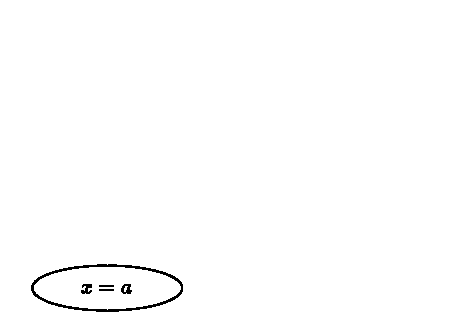
\includegraphics[]{images/x_a/x_a-1.pdf}
\end{frame}

\begin{frame}{Satisfiable Example $x = a$}
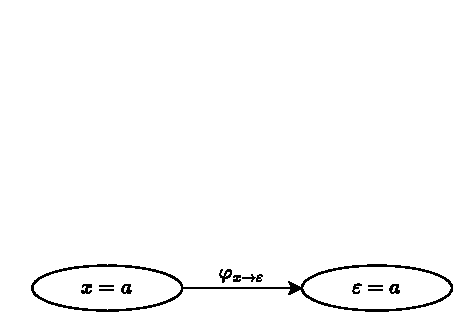
\includegraphics[]{images/x_a/x_a-2.pdf}
\end{frame}

\begin{frame}{Satisfiable Example $x = a$}
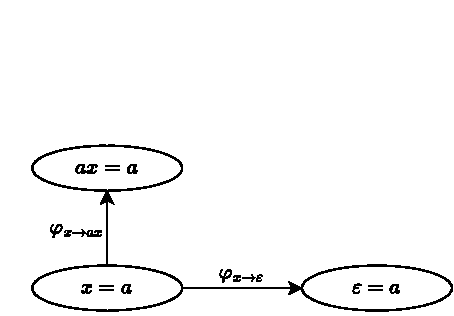
\includegraphics[]{images/x_a/x_a-3.pdf}
\end{frame}

\begin{frame}{Satisfiable Example $x = a$}
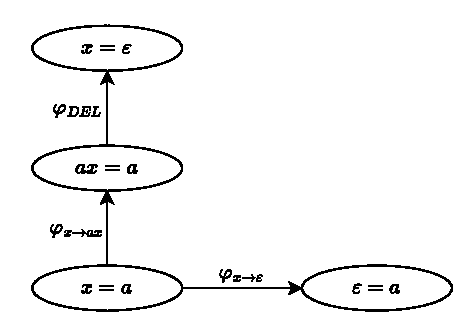
\includegraphics[]{images/x_a/x_a-4.pdf}
\end{frame}

\begin{frame}{Satisfiable Example $x = a$}
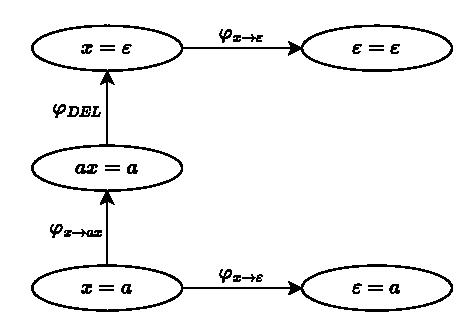
\includegraphics[]{images/x_a/x_a-5.pdf}
\end{frame}

\begin{frame}{Satisfiable Example $x = a$}
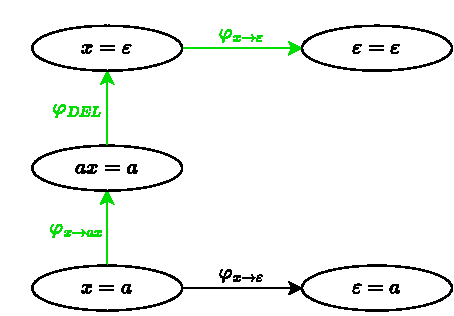
\includegraphics[]{images/x_a/x_a-6.pdf}
\end{frame}

\begin{frame}{Unsatisfiable Example $xa = bx$}
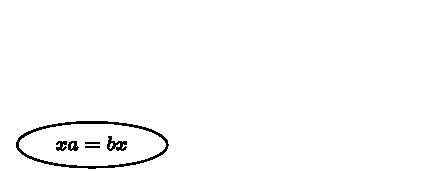
\includegraphics[]{images/xa_bx/xa_bx-0.pdf}
\end{frame}

\begin{frame}{Unsatisfiable Example $xa = bx$}
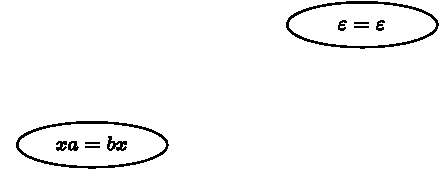
\includegraphics[]{images/xa_bx/xa_bx-1.pdf}
\end{frame}

\begin{frame}{Unsatisfiable Example $xa = bx$}
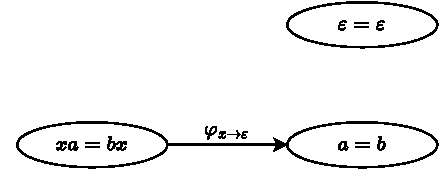
\includegraphics[]{images/xa_bx/xa_bx-2.pdf}
\end{frame}

\begin{frame}{Unsatisfiable Example $xa = bx$}
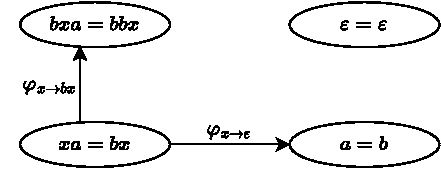
\includegraphics[]{images/xa_bx/xa_bx-3.pdf}
\end{frame}

\begin{frame}{Unsatisfiable Example $xa = bx$}
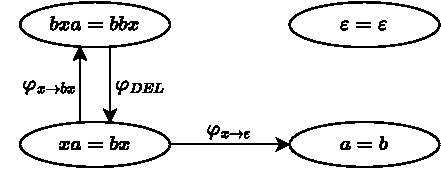
\includegraphics[]{images/xa_bx/xa_bx-4.pdf}
\end{frame}

\begin{frame}{Unsatisfiable Example $xa = bx$}
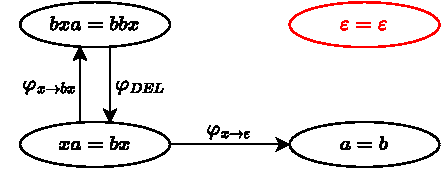
\includegraphics[]{images/xa_bx/xa_bx-5.pdf}
\end{frame}

\begin{frame}{Regular Expressions}
\pause
$ab*$\pause$, L(ab*) = \{a, ab, abb, ...\}$ \\

\begin{outline}
    \pause
    \1 $a$, $L(a) = \{a\}$
    \pause
    \1 $\lambda$, $L(\lambda) = \{\varepsilon\}$
    \pause
    \1 $\emptyset$, $L(\emptyset) = \{\}$
\end{outline}

\pause
For regular expressions $p, q$
\begin{outline}
    \pause
    \1 $pq$
    \pause
    \1 $p*$, $L(p*) = \{\varepsilon, p, pp, ppp, ...\}$
    \pause
    \1 $p', p\&q, p|q$
\end{outline}
\end{frame}

\begin{frame}{Brzozowski Derivatives}
Observation: $a\alpha \in L(ap) \Leftrightarrow \alpha \in L(p)$ \\
\pause
$D$\pause$_a$\pause$(ap)$ \pause $= p$ \\
\pause
$D_aq =\:?$\pause, s.t. $L(D_aq) = \{\alpha\:|\:\forall a\alpha \in L(q)\}$ 
\end{frame}

\begin{frame}{Example}
\begin{tabular}{c l l}
     & $ab$&$\in L(a(b|c))$ \\
     \pause
    $\Leftrightarrow$ & $b$&$\in L(D_a(a(b|c)))$ \pause $= L(b|c)$ \\
    \pause
    $\Leftrightarrow$ & $\varepsilon$&$\in L(D_b(b|c))$ \pause $= L(\lambda|\emptyset)$\\
    \pause
    $\Leftrightarrow$ & $true$ & \\
\end{tabular}

\pause
~\\

$a_1a_2...a_n \in L(p)$ \pause $\Leftrightarrow \varepsilon \in L(D_{a_n}(...(D_{a_2}(D_{a_1}p))))$
\end{frame}

\begin{frame}{Regex Nullability}

\pause
We define $\nu(p) :\Leftrightarrow \varepsilon \in L(p)$\\

\begin{tabular}{l c c}
    \pause
    $\nu(\lambda)$ & $=$ & $true$ \\
    \pause
    $\nu(\emptyset)$ & $=$ & $false$ \\
    \pause
    $\nu(a)$ & $=$ & $false$ \\
    \pause
    $\nu(pq)$ & $=$ & $\nu(p) \land \nu(q)$ \\
    \pause
    $\nu(p*)$ & $=$ & $true$ \\
    \pause
    & ... & \\
\end{tabular}
\end{frame}

\begin{frame}{Regex Satisfiability}

\pause
We define $\sigma(p) :\Leftrightarrow L(p) \neq \{\}$\\

\begin{tabular}{l c c}
    \pause
    $\sigma(\emptyset)$ & $=$ & $false$ \\
    \pause
    $\sigma(\lambda)$ & $=$ & $true$ \\
    \pause
    $\sigma(a)$ & $=$ & $true$ \\
    \pause
    $\sigma(pq)$ & $=$ & $\sigma(p) \land \sigma(q)$ \\
    \pause
    & ... & \\
\end{tabular}
\end{frame}

\begin{frame}{Regex Derivative}

We define $D_ap$\\

\begin{tabular}{l c l}
    \pause
    $D_aa$ & $=$ & $\lambda$ \\
    \pause
    $D_ab$ & $=$ & $\emptyset$ \\
    \pause
    $D_a\lambda$ & $=$ & $\emptyset$ \\
    \pause
    $D_a\emptyset$ & $=$ & $\emptyset$ \\
    \pause

    $D_a(pq)$ & $=$ & $
    \left\{
	\begin{array}{ll}
		(D_ap)q\:|\:D_aq  & \mbox{if } \nu(p) \\
		(D_ap)q & \mbox{if } \neg \nu(p)
	\end{array}
    \right.
    $ \\
    \pause
    
    $D_a(p*)$ & $=$ & $(D_ap)p*$ \\
    \pause
    & ... & \\
\end{tabular}
\end{frame}

\section{Approach}
\begin{frame}{Modified Algorithm}
\pause
$a, b \in \Sigma, a \neq b, x, y \in X, x \neq y, \alpha, \beta \in (\Sigma \cup X)^*$\pause{\color{green}$, c(x), c(y)$ regex constraints} \\

\begin{enumerate}
    \pause
    \item $a\alpha = a\beta \rightarrow \varphi_{DEL}$
    \pause
    \item $a\alpha = b\beta \rightarrow$ \xmark
    \pause
    \item $x\alpha = \beta \rightarrow \varphi_{x \rightarrow \varepsilon}$\pause, {\color{green}if $\nu(c(x))$}
    \pause
    \item $x\alpha = a\beta \rightarrow \varphi_{x \rightarrow ax'}$\pause,
    {\color{green}if $\sigma(D_a(c(x))$\pause, introduce $c(x') := D_a(c(x))$}
    \pause
    \item $x\alpha = x\beta \rightarrow \varphi_{DEL}$\pause,
    {\color{green}if $\sigma(c(x))$}
    \pause
    \item $x\alpha = y\beta$\pause,
    {\color{green}???}
\end{enumerate}

\end{frame}

\begin{frame}{Case 6 - Prefix fetching}
$x\alpha = y\beta$

\pause
common prefix $a \in \Sigma$, s.t. $\sigma(D_a(c(x))), \sigma(D_a(c(y)))$

\pause
rewrite $\varphi_{y \rightarrow ay'}$\pause, introduce $c(y') := D_a(c(y))$
\end{frame}


\section{Implementation}
\begin{frame}{Implementation}
\pause
\centering
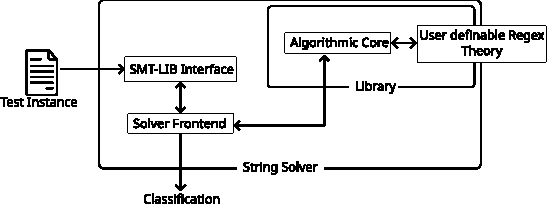
\includegraphics[]{images/architecture.pdf}
\end{frame}

\begin{frame}[fragile]{Implementation}
\begin{minted}{haskell}
class RegexTheory r where
    derive :: Char -> r -> r
    nullable :: r -> Bool
    satisfiable :: r -> Bool
\end{minted}

\pause
~\\

\begin{minted}{haskell}
nielsen :: RegexTheory r => Equation r -> Bool
\end{minted}
\end{frame}

\section{Benchmarks}
\begin{frame}{Benchmarks}
\begin{itemize}
    \pause
    \item benchmarkset-1 (quadratic, regex)
    \pause
    \item benchmarkset-2 (quadratic)
    \pause
    \item benchmarkset-2\:\textbackslash\:benchmarkset-1 (quadratic, non-regex)
\end{itemize}
    
\end{frame}

\begin{frame}{Solvers}
\begin{itemize}
    \pause
    \item CVC4, CVC5
    \pause
    \item Z3Seq, Z3str3
    \pause
    \item Woorpje, Woorpje-levis
    \pause
    \item Noodler
    \pause
    \item nielsen-transformation (nt)
\end{itemize}
\end{frame}

\begin{frame}{Solvers}
\resizebox{1 \textwidth}{!}{
\begin{tabular}{|c|c|c|c|c|}
    \hline
    Solver & Version & State of the art & Can solve regex & Combined solving \\
    \hline
    CVC4                   &    1.8 & \cellcolor{green!25}\cmark & \cellcolor{green!25}\cmark &
    \cellcolor{red!25}\xmark \\
    \hline
    CVC5                   &  1.0.3 & \cellcolor{green!25}\cmark & \cellcolor{green!25}\cmark &
    \cellcolor{red!25}\xmark \\
    \hline
    Z3Seq                  & 4.8.10 & \cellcolor{green!25}\cmark & \cellcolor{green!25}\cmark &
    \cellcolor{red!25}\xmark \\
    \hline
    Z3str3                 & 4.8.10 & \cellcolor{green!25}\cmark & \cellcolor{green!25}\cmark &
    \cellcolor{red!25}\xmark \\
    \hline
    woorpje                & spin22 &   \cellcolor{red!25}\xmark & \cellcolor{green!25}\cmark &
    \cellcolor{red!25}\xmark \\
    \hline
    woorpje-levi           & spin22 &   \cellcolor{red!25}\xmark &   \cellcolor{red!25}\xmark &
    \cellcolor{red!25}\xmark \\
    \hline
    noodler                & f752e79 &   \cellcolor{red!25}\xmark & \cellcolor{green!25}\cmark &
    \cellcolor{green!25}\cmark \\
    \hline
    nielsen-transformation &  0.1.0 &   \cellcolor{red!25}\xmark & \cellcolor{green!25}\cmark &
    \cellcolor{green!25}\cmark \\
    \hline
\end{tabular}
}
\end{frame}

\section{Results}
\begin{frame}{Results}
\end{frame}

\begin{frame}{benchmarkset-1}
\resizebox{\textwidth}{!}{
\begin{tabular}{c|r|r|r|r|r|r|r}
Solver & Satis & NSatis & Unknown & Timeout & Errors & Total Time & Total Time w/o Timeout\\
\hline
CVC4 & 747 & 1400 & 0 & 0 & 0 & 240297 & 240297\\
CVC5 & 747 & 1400 & 0 & 0 & 0 & 247331 & 247331\\
Z3seq & 748 & 1398 & 0 & 1 & 55 & 865382 & 845382\\
Z3str3 & 748 & 1398 & 0 & 1 & 55 & 950974 & 930974\\
woorpje & 393 & 643 & 684 & 427 & 126 & 13319883 & 4779883\\
noodler & 243 & 824 & 637 & 443 & 0 & 27816800 & 18956584\\
nielsen-transformation & 747 & 1398 & 0 & 2 & 0 & 251808 & 211808\\
\end{tabular}
}
\end{frame}

\begin{frame}{benchmarkset-1}
\resizebox{\textwidth}{!}{
\begin{tabular}{c|r|r|r|r|r|r|r}
Solver & Satis & NSatis & Unknown & Timeout & Errors & Total Time & Total Time w/o Timeout\\
\hline
CVC4 & \cellcolor{blue!25}747 & \cellcolor{blue!25}1400 & 0 & 0 & 0 & 240297 & 240297\\
CVC5 & \cellcolor{blue!25}747 & \cellcolor{blue!25}1400 & 0 & 0 & 0 & 247331 & 247331\\
Z3seq & 748 & 1398 & 0 & 1 & 55 & 865382 & 845382\\
Z3str3 & 748 & 1398 & 0 & 1 & 55 & 950974 & 930974\\
woorpje & 393 & 643 & 684 & 427 & 126 & 13319883 & 4779883\\
noodler & 243 & 824 & 637 & 443 & 0 & 27816800 & 18956584\\
nielsen-transformation & \cellcolor{blue!25}747 & \cellcolor{blue!25}1398 & 0 & 2 & 0 & 251808 & 211808\\
\end{tabular}
}
\end{frame}


\begin{frame}{benchmarkset-1}
\resizebox{\textwidth}{!}{
\begin{tabular}{c|r|r|r|r|r|r|r}
Solver & Satis & NSatis & Unknown & Timeout & Errors & Total Time & \cellcolor{blue!25}Total Time w/o Timeout\\
\hline
CVC4 & 747 & 1400 & 0 & 0 & 0 & 240297 & \cellcolor{blue!25}240297\\
CVC5 & 747 & 1400 & 0 & 0 & 0 & 247331 & \cellcolor{blue!25}247331\\
Z3seq & 748 & 1398 & 0 & 1 & 55 & 865382 & \cellcolor{blue!25}845382\\
Z3str3 & 748 & 1398 & 0 & 1 & 55 & 950974 & \cellcolor{blue!25}930974\\
woorpje & 393 & 643 & 684 & 427 & 126 & 13319883 & \cellcolor{blue!25}4779883\\
noodler & 243 & 824 & 637 & 443 & 0 & 27816800 & \cellcolor{blue!25}18956584\\
nielsen-transformation & 747 & 1398 & 0 & 2 & 0 & 251808 & \cellcolor{blue!25}211808\\
\end{tabular}
}
\end{frame}

\begin{frame}{benchmarkset-1}
\begin{figure}%[H]
\begin{center}
\resizebox{0.6 \textwidth}{!}{
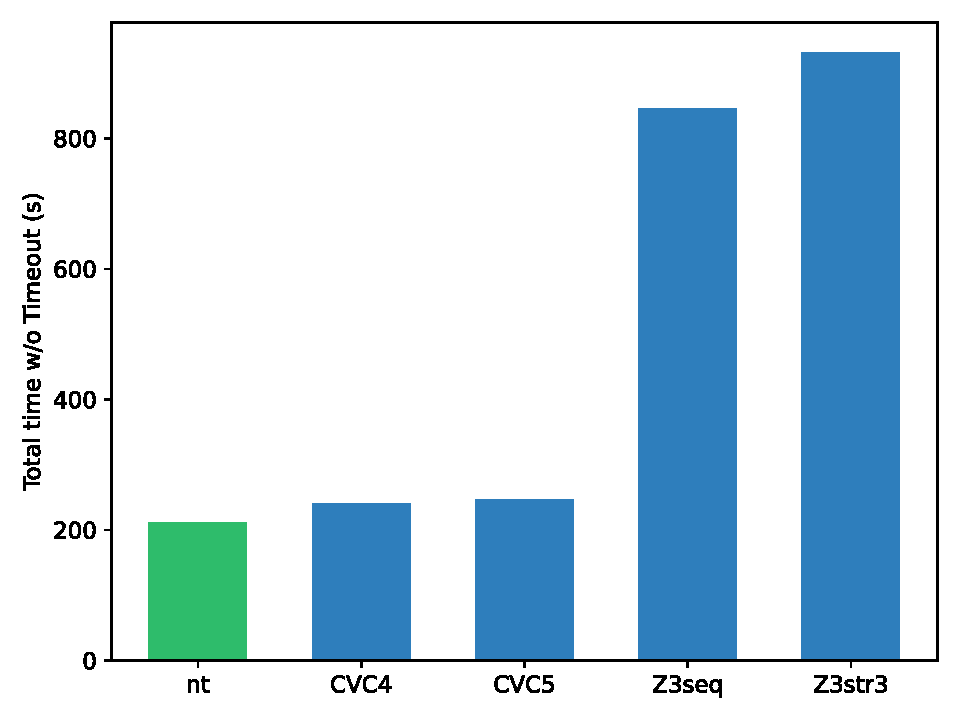
\includegraphics[]{images/bar-1.pdf}
}
\end{center}
\end{figure}
\end{frame}

\begin{frame}{benchmarkset-2}
\resizebox{\textwidth}{!}{
\begin{tabular}{c|r|r|r|r|r|r|r}
Solver & Satis & NSatis & Unknown & Timeout & Errors & Total Time & Total Time w/o Timeout\\
\hline
CVC4 & 1055 & 1491 & 0 & 1 & 0 & 326543 & 306543\\
CVC5 & 1055 & 1491 & 0 & 1 & 0 & 354380 & 334380\\
Z3seq & 1045 & 1409 & 0 & 93 & 55 & 2908422 & 1048422\\
Z3str3 & 1057 & 1408 & 5 & 77 & 55 & 2571637 & 1031637\\
woorpje & 693 & 651 & 695 & 508 & 127 & 15410164 & 5250164\\
noodler & 544 & 888 & 665 & 450 & 0 & 32926399 & 23926181\\
nielsen-transformation & 1011 & 1453 & 0 & 83 & 0 & 2371652 & 711652\\
\end{tabular}
}
\end{frame}

\begin{frame}{benchmarkset-2}
\resizebox{\textwidth}{!}{
\begin{tabular}{c|r|r|r|r|r|r|r}
Solver & Satis & NSatis & Unknown & Timeout & Errors & Total Time & \cellcolor{blue!25}Total Time w/o Timeout\\
\hline
CVC4 & 1055 & 1491 & 0 & 1 & 0 & 326543 & \cellcolor{blue!25}306543\\
CVC5 & 1055 & 1491 & 0 & 1 & 0 & 354380 & \cellcolor{blue!25}334380\\
Z3seq & 1045 & 1409 & 0 & 93 & 55 & 2908422 & \cellcolor{blue!25}1048422\\
Z3str3 & 1057 & 1408 & 5 & 77 & 55 & 2571637 & \cellcolor{blue!25}1031637\\
woorpje & 693 & 651 & 695 & 508 & 127 & 15410164 & \cellcolor{blue!25}5250164\\
noodler & 544 & 888 & 665 & 450 & 0 & 32926399 & \cellcolor{blue!25}23926181\\
nielsen-transformation & 1011 & 1453 & 0 & 83 & 0 & 2371652 & \cellcolor{blue!25}711652\\
\end{tabular}
}
\end{frame}

\begin{frame}{benchmarkset-2}
\begin{figure}%[H]
\begin{center}
\resizebox{0.6 \textwidth}{!}{
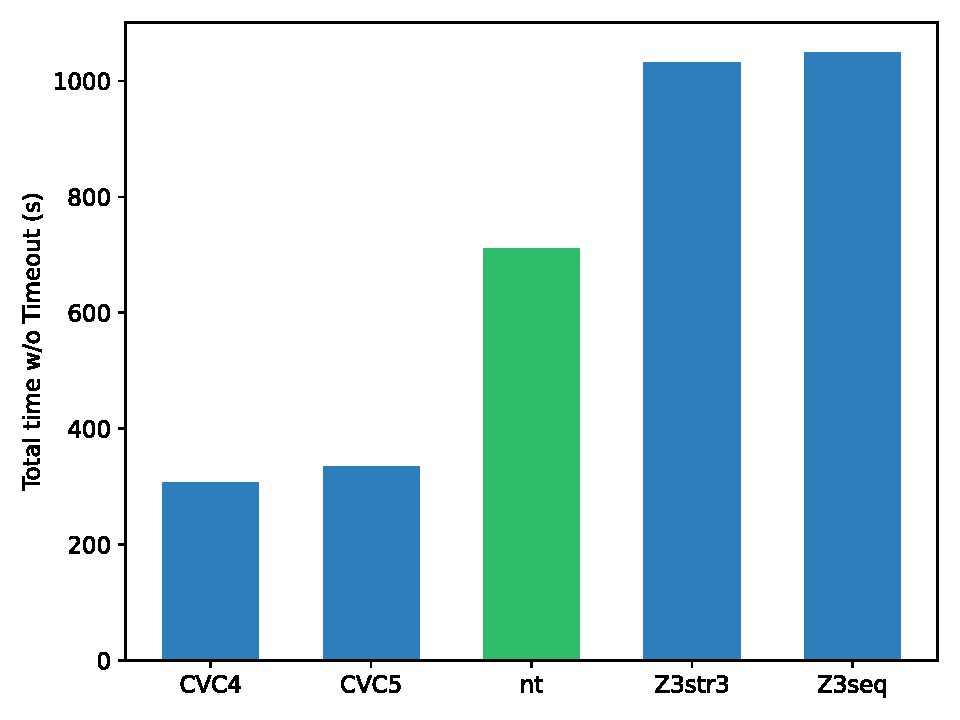
\includegraphics[]{images/bar-2.pdf}
}
\end{center}
\end{figure}
\end{frame}

\begin{frame}{benchmarkset-2\:\textbackslash\:benchmarkset-1}
\resizebox{\textwidth}{!}{
\begin{tabular}{c|r|r|r|r|r|r|r}
Solver & Satis & NSatis & Unknown & Timeout & Errors & Total Time & Total Time w/o Timeout\\
\hline
CVC4 & 308 & 91 & 0 & 1 & 0 & 90983 & 70983\\
CVC5 & 308 & 91 & 0 & 1 & 0 & 110981 & 90981\\
Z3seq & 297 & 11 & 0 & 92 & 0 & 2085124 & 245124\\
Z3str3 & 309 & 10 & 5 & 76 & 0 & 1643121 & 123121\\
woorpje & 299 & 4 & 8 & 89 & 0 & 2464010 & 684010\\
woorpje-levis & 300 & 90 & 9 & 1 & 1 & 206817 & 186817\\
noodler & 281 & 20 & 19 & 80 & 0 & 5256067 & 3656067\\
nielsen-transformation & 264 & 54 & 0 & 82 & 0 & 2111959 & 471959\\
\end{tabular}
}
\end{frame}

\begin{frame}{benchmarkset-2\:\textbackslash\:benchmarkset-1}
\resizebox{\textwidth}{!}{
\begin{tabular}{c|r|r|r|r|r|r|r}
Solver & Satis & NSatis & Unknown & Timeout & Errors & Total Time & Total Time w/o Timeout\\
\hline
CVC4 & 308 & 91 & 0 & 1 & 0 & 90983 & 70983\\
CVC5 & 308 & 91 & 0 & 1 & 0 & 110981 & 90981\\
Z3seq & 297 & 11 & 0 & 92 & 0 & 2085124 & 245124\\
Z3str3 & 309 & 10 & 5 & 76 & 0 & 1643121 & 123121\\
woorpje & 299 & 4 & 8 & 89 & 0 & 2464010 & \cellcolor{blue!25}684010\\
woorpje-levis & 300 & 90 & 9 & 1 & 1 & 206817 & \cellcolor{blue!25}186817\\
noodler & 281 & 20 & 19 & 80 & 0 & 5256067 & 3656067\\
nielsen-transformation & 264 & 54 & 0 & 82 & 0 & 2111959 & 471959\\
\end{tabular}
}
\end{frame}

\begin{frame}{benchmarkset-2\:\textbackslash\:benchmarkset-1}
\resizebox{\textwidth}{!}{
\begin{tabular}{c|r|r|r|r|r|r|r}
Solver & Satis & NSatis & Unknown & Timeout & Errors & Total Time & Total Time w/o Timeout\\
\hline
CVC4 & 308 & 91 & 0 & 1 & 0 & 90983 & 70983\\
CVC5 & 308 & 91 & 0 & 1 & 0 & 110981 & 90981\\
Z3seq & 297 & 11 & 0 & 92 & 0 & 2085124 & 245124\\
Z3str3 & 309 & 10 & 5 & 76 & 0 & 1643121 & 123121\\
woorpje & 299 & 4 & 8 & 89 & 0 & 2464010 & 684010\\
woorpje-levis & 300 & 90 & 9 & 1 & 1 & 206817 & \cellcolor{blue!25}186817\\
noodler & 281 & 20 & 19 & 80 & 0 & 5256067 & 3656067\\
nielsen-transformation & 264 & 54 & 0 & 82 & 0 & 2111959 & \cellcolor{blue!25}471959\\
\end{tabular}
}
\end{frame}

\begin{frame}{benchmarkset-2\:\textbackslash\:benchmarkset-1}
\resizebox{\textwidth}{!}{
\begin{tabular}{c|r|r|r|r|r|r|r}
Solver & Satis & NSatis & Unknown & Timeout & Errors & Total Time & \cellcolor{blue!25}Total Time w/o Timeout\\
\hline
CVC4 & 308 & 91 & 0 & 1 & 0 & 90983 & \cellcolor{blue!25}70983\\
CVC5 & 308 & 91 & 0 & 1 & 0 & 110981 & \cellcolor{blue!25}90981\\
Z3seq & 297 & 11 & 0 & 92 & 0 & 2085124 & \cellcolor{blue!25}245124\\
Z3str3 & 309 & 10 & 5 & 76 & 0 & 1643121 & \cellcolor{blue!25}123121\\
woorpje & 299 & 4 & 8 & 89 & 0 & 2464010 & \cellcolor{blue!25}684010\\
woorpje-levis & 300 & 90 & 9 & 1 & 1 & 206817 & \cellcolor{blue!25}186817\\
noodler & 281 & 20 & 19 & 80 & 0 & 5256067 & \cellcolor{blue!25}3656067\\
nielsen-transformation & 264 & 54 & 0 & 82 & 0 & 2111959 & \cellcolor{blue!25}471959\\
\end{tabular}
}
\end{frame}

\begin{frame}{benchmarkset-2\:\textbackslash\:benchmarkset-1}
\begin{figure}%[H]
\begin{center}
\resizebox{0.6 \textwidth}{!}{
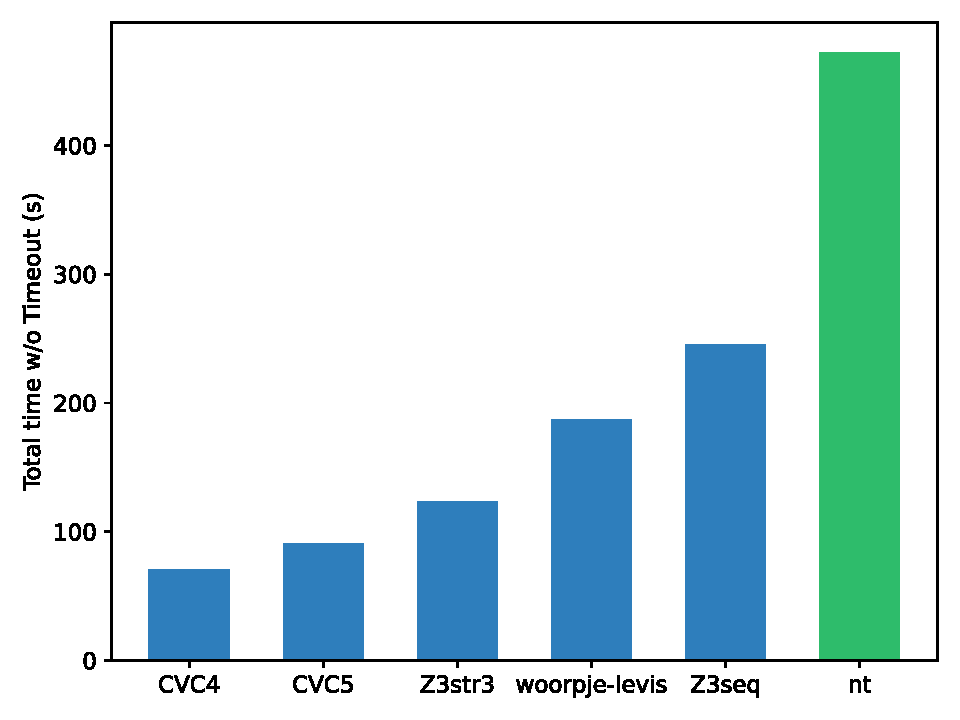
\includegraphics[]{images/bar-2-without-1.pdf}
}
\end{center}
\end{figure}
\end{frame}


\begin{frame}{Summary}

\begin{figure}[htp]

\centering
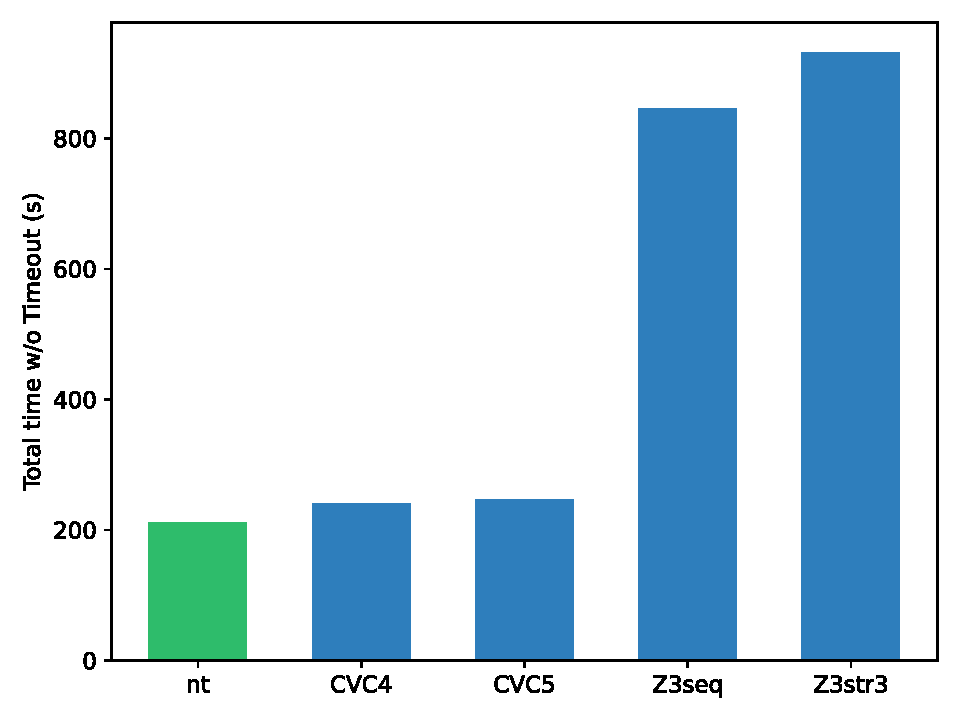
\includegraphics[width=.33\textwidth]{images/bar-1.pdf}\hfill
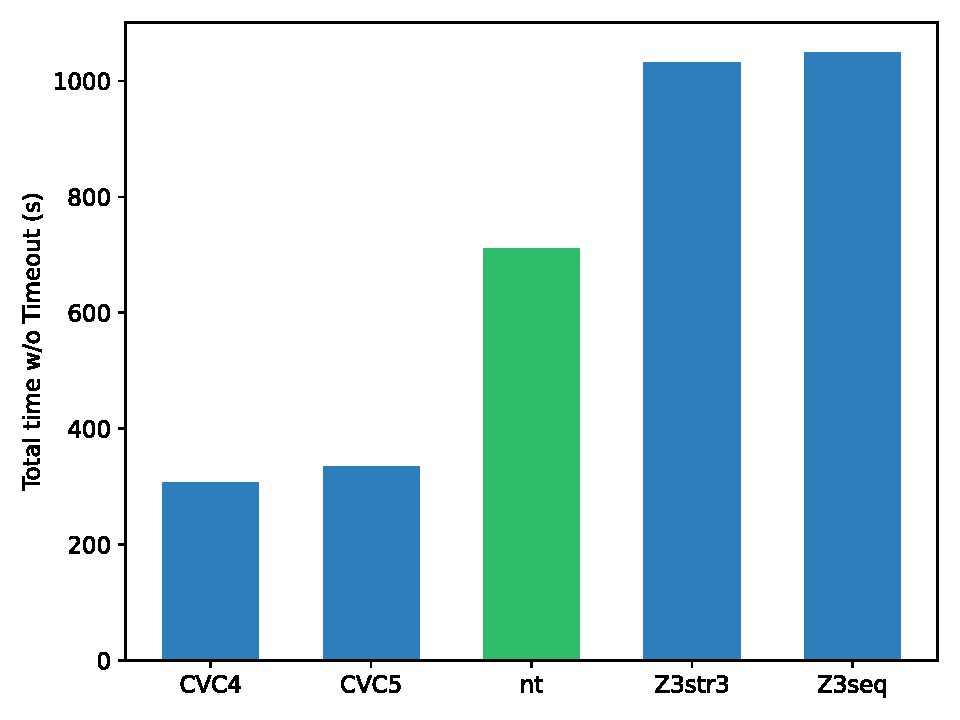
\includegraphics[width=.33\textwidth]{images/bar-2.pdf}\hfill
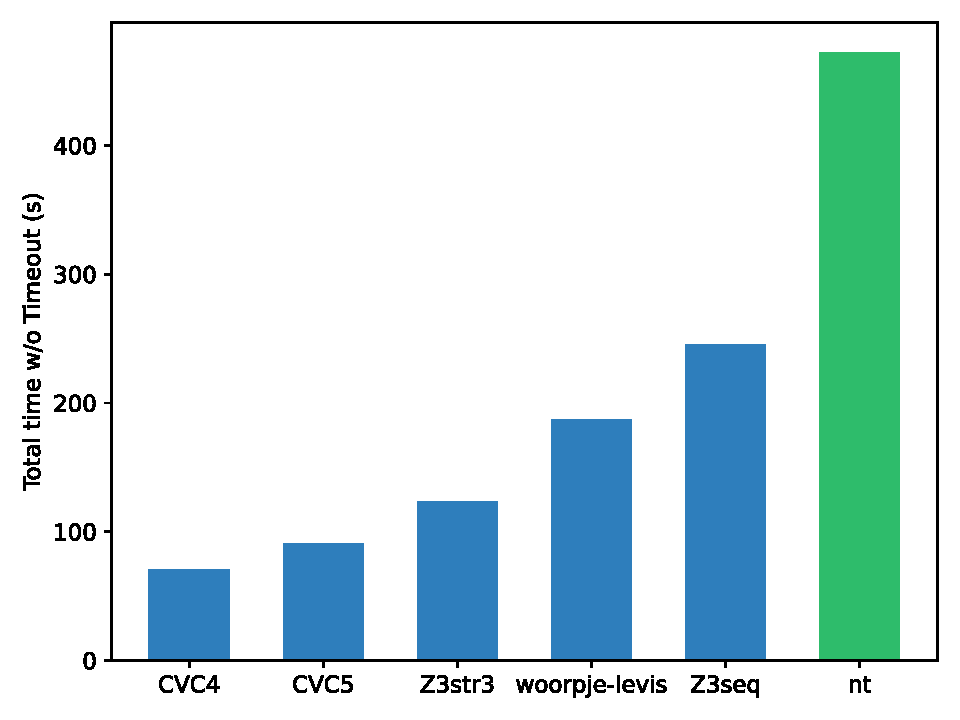
\includegraphics[width=.33\textwidth]{images/bar-2-without-1.pdf}

\end{figure}
% \begin{tabular}{c c c}
% 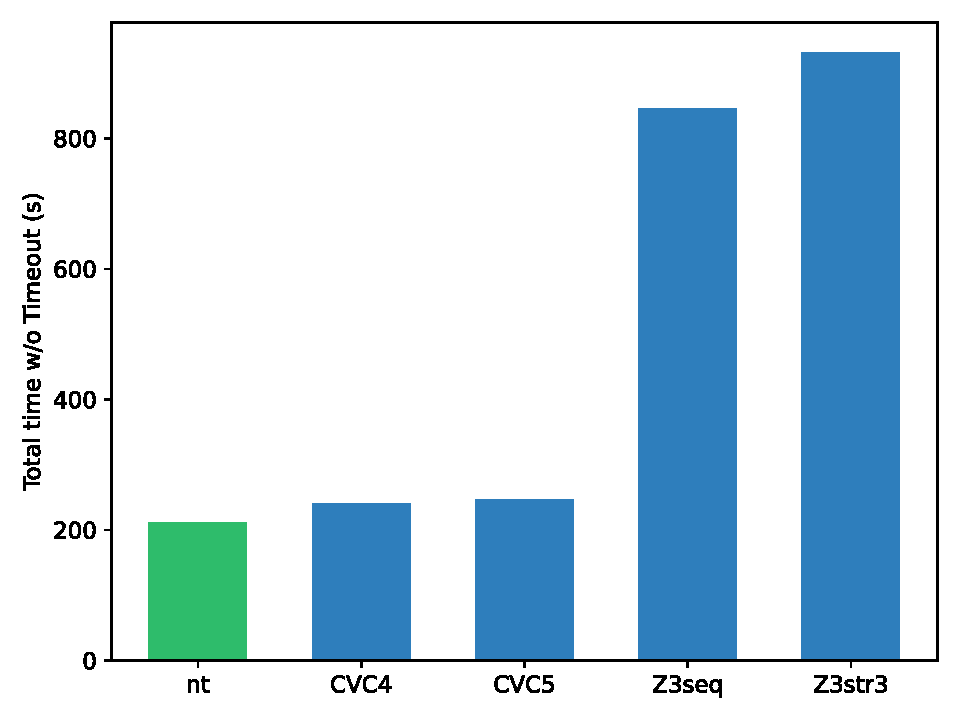
\includegraphics[width=.3\textwidth]{images/bar-1.pdf}\hfill
% &
% 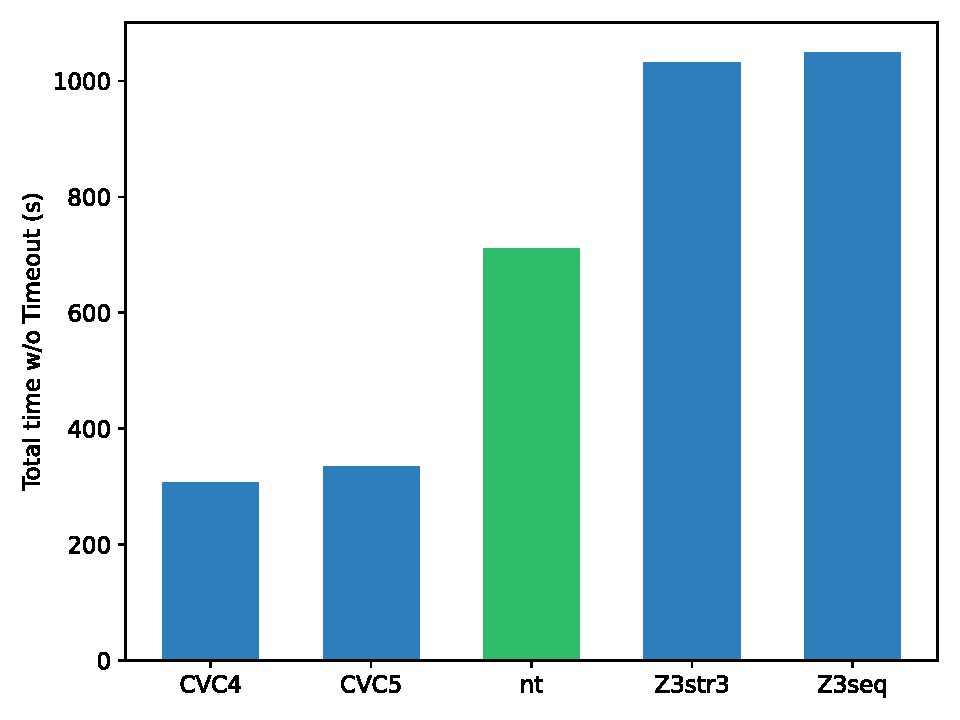
\includegraphics[width=.3\textwidth]{images/bar-2.pdf}\hfill
% &
% 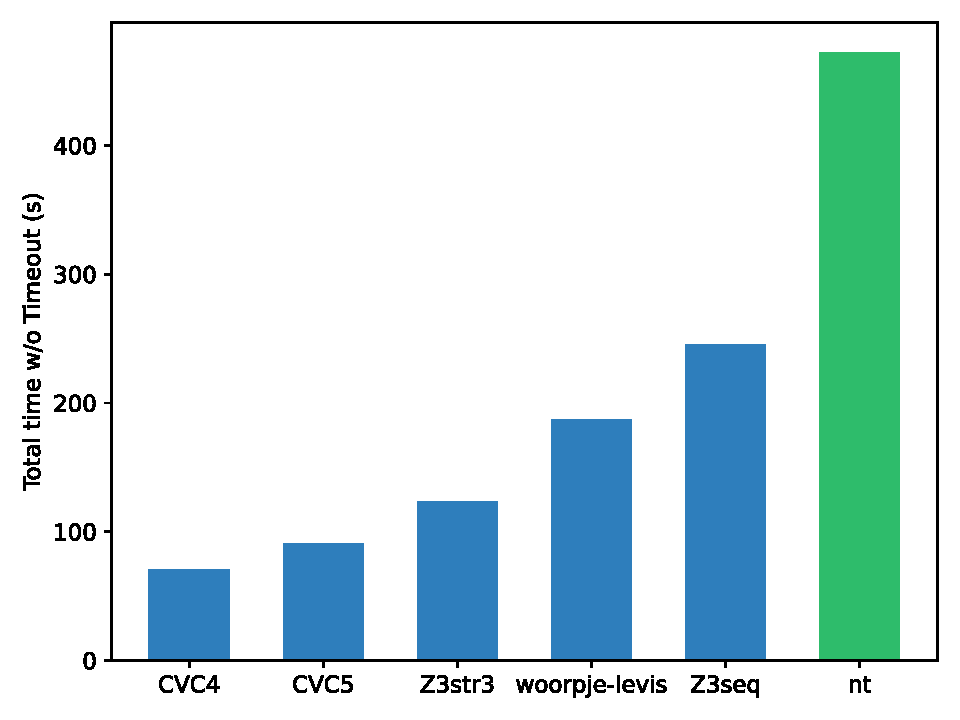
\includegraphics[width=.3\textwidth]{images/bar-2-without-1.pdf}
% \end{tabular}
% \\
% benchmarkset-1 & benchmarkset-2 & 
% benchmarkset-2 - benchmarkset-1
% \\

\end{frame}


\end{document}